% CMPE 249 final report. Build: tectonic report/main.tex  (or latexmk -pdf main.tex)
% Numbers marked \pending{} are filled in when the Nov 27 runs finish (see hpc/plan.txt).
\documentclass[conference]{IEEEtran}
\usepackage{graphicx,booktabs,amsmath,amssymb,xcolor,tikz,url}
\usepackage[hidelinks]{hyperref}
\usetikzlibrary{arrows.meta,positioning}
\graphicspath{{figures/}}
\newcommand{\pending}[1]{\textcolor{red}{[#1]}}

\begin{document}
\title{Does the Source of Exploration Data Matter\\for Fine-Tuning a Small Vision-Language-Action Model?}
\author{\IEEEauthorblockN{Aaron Chandler}
\IEEEauthorblockA{CMPE 249 Intelligent Autonomous Systems, San Jos\'e State University\\
Code: \url{https://github.com/AaronChandler976/curious-vla} \quad Video: \pending{link}}}
\maketitle

\begin{abstract}
Vision-language-action (VLA) policies learn manipulation from teleoperated demonstrations, which are expensive, while a robot can collect task-free exploration data at almost no cost. Prior work shows that exploration data can help VLA post-training through reinforcement learning or inverse-dynamics pretraining, but not whether the \emph{source} of that data matters when it is added to ordinary behavior-cloning fine-tuning. We fine-tune SmolVLA (450M parameters) on two LIBERO-Object tasks with 10, 25 or 40 demonstrations per task and compare three conditions under matched budgets: demonstrations only, demonstrations plus random exploration, and demonstrations plus curiosity-driven (ICM) exploration, at 5k and 20k exploration steps, with 10 training seeds per cell and \pending{464} fine-tunes in total. No exploration mix beats demonstrations only: pooled over demonstration budgets, mixing in exploration changes success by $-14$ to $-6$ points (random) and $-19$ to $-2$ points (ICM). The ICM-versus-random difference reverses sign between budgets (+12 and $-13$ points) and is as large as the variation between independent collections of the same method. Diagnostics show why: SmolVLA trains only its action expert, and exploration actions cannot be predicted from observations (held-out $R^2\le0.01$ versus 0.42 for demonstrations), so the behavior-cloning loss can only learn noise from them. Falsification tests separate dilution from active harm, test exploration-first training, and test a properly trained curiosity explorer \pending{results}. The practical conclusion is that task-free exploration data should not be co-trained into a VLA with a behavior-cloning loss; how the data is used matters more than which explorer collected it.
\end{abstract}

\section{Introduction}
Demonstrations for robot manipulation are collected by teleoperation, one task at a time. A robot left to explore on its own produces far more interaction data for free, but that data carries no task instruction and no reward. Whether such data can substitute for demonstrations is an open question for vision-language-action (VLA) models, which are now the standard way to map images and an instruction to robot actions.

Two recent results show that exploration data \emph{can} help a VLA. World-Env~\cite{worldenv} collects exploration from a perturbed, already-trained policy and uses it for reinforcement learning inside a learned world model. TAP~\cite{tap} pretrains a VLA on 30 hours of random robot play with an inverse-dynamics objective and gains 10 points on SIMPLER. Neither compares exploration \emph{sources}, and neither tests the simplest way a practitioner would use the data: adding it to the behavior-cloning (BC) fine-tuning set. ExORL~\cite{exorl} showed that the choice of explorer matters a great deal for offline reinforcement learning, but that setting relabels the data with rewards, which VLA fine-tuning does not have.

This project asks: \emph{at the same amount of collected data, does curiosity-driven exploration give a small VLA more downstream value than random exploration, or than no exploration at all?} Contributions:
\begin{itemize}
\item A reproducible, offline HPC pipeline for SmolVLA on LIBERO in which every condition shares one data path and every training frame is verified against its source.
\item A controlled comparison of demos-only, demos+random and demos+ICM fine-tuning over 3 demonstration budgets, 2 exploration budgets and 10 seeds, with hierarchical-bootstrap and paired statistics.
\item A negative result with a diagnosis: exploration data mixed into BC fine-tuning never helps, and the apparent ICM-versus-random effect is within the variation between data collections.
\item Falsification tests that separate dilution from harm, test exploration-first training, and test a trained curiosity explorer.
\end{itemize}

\section{Related Work}
\textbf{VLA models.} OpenVLA, $\pi_0$ and SmolVLA~\cite{smolvla} map images, robot state and an instruction to actions; SmolVLA uses a frozen SmolVLM2 backbone and a flow-matching action expert that predicts 50-step action chunks. LIBERO~\cite{libero} is the standard simulated benchmark for fine-tuning them.

\textbf{Exploration data for VLAs.} World-Env~\cite{worldenv} uses perturbed-policy exploration for RL post-training in a world model. TAP~\cite{tap} uses random play for inverse-dynamics pretraining. DLR~\cite{dlr} generates diverse trajectories with RL for VLA pretraining on LIBERO. Prompt-driven exploration and ExToken explore within VLA reinforcement learning rather than producing data.

\textbf{Curiosity and data for offline learning.} ICM~\cite{icm} rewards an agent for transitions its forward model cannot predict. ExORL~\cite{exorl} collects reward-free data with ICM, RND, APT and others and shows that the data source drives offline-RL performance. SENSEI~\cite{sensei} uses VLM judgments of interestingness to guide exploration.

\textbf{Mixed-quality data.} Action-only pretraining on heterogeneous robot data is fragile, and language supervision and future-latent alignment make transfer more stable~\cite{negtransfer}; failed rollouts help when used as negatives or recovery data rather than as imitation targets~\cite{fact}.

\section{Method}
\subsection{Problem formulation}
Let $\mathcal{D}_n$ be $n$ demonstrations per task for tasks $T=\{0,1\}$ of LIBERO-Object, and $\mathcal{E}_m^{s}$ the first $m$ environment steps collected by explorer $s\in\{\text{random},\text{ICM}\}$ in the same scenes, without task labels or rewards. A policy $\pi_\theta(a_{t:t+49}\mid o_t, \ell)$ maps camera images, the 8-D robot state and an instruction $\ell$ to a 7-D action chunk. We fine-tune $\pi_\theta$ on $\mathcal{D}_n$ alone or on $\mathcal{D}_n\cup\mathcal{E}_m^{s}$ with a fixed number of gradient steps, and measure task success over 50 rollouts per task. The quantity of interest is the change in success per unit of collected exploration data, $\Delta_s(n,m)=\mathrm{SR}(\mathcal{D}_n\cup\mathcal{E}^s_m)-\mathrm{SR}(\mathcal{D}_n)$, and the source effect $\Delta_{\text{ICM}}-\Delta_{\text{random}}$.

\subsection{System}
Fig.~\ref{fig:arch} shows the pipeline. Explorers act in the same two LIBERO-Object scenes as the demonstrations and record every step through LeRobot's LIBERO wrapper, so observations (two $256\times256$ cameras rotated as in the demonstrations, 8-D state) and actions (7-D, gripper $\pm1$) have exactly the demonstration format, which a format check verifies. A builder writes each training set as a fresh LeRobot dataset from raw parquet rows (demonstrations only, a mix, or exploration only), and a verifier loads it exactly as the trainer does and compares sampled frames, 50-step action chunks and instructions with the source rows. A dry run executes every code path on CPU before any GPU job is queued. On the cluster, a cron-driven autopilot submits every run in the experiment plan, resubmits jobs that land on faulty nodes, and refreshes the analysis.

\begin{figure}[t]\centering
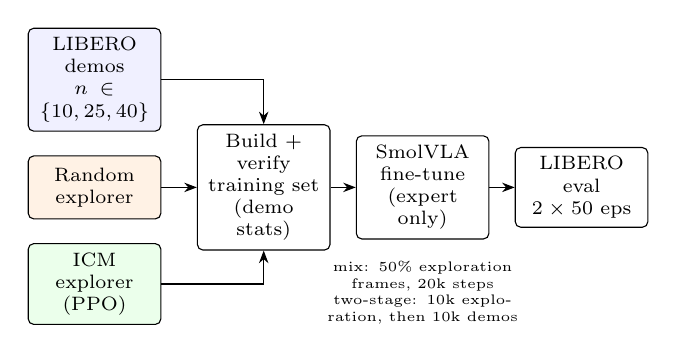
\begin{tikzpicture}[font=\scriptsize, node distance=0.3cm and 0.32cm,
 box/.style={draw, rounded corners=2pt, align=center, minimum height=0.8cm, text width=1.45cm, fill=white},
 data/.style={box, fill=blue!6}, arr/.style={-{Stealth[length=1.6mm]}}]
\node[data] (d) {LIBERO demos\\$n\in\{10,25,40\}$};
\node[box, below=of d, fill=orange!10] (r) {Random\\explorer};
\node[box, below=of r, fill=green!8] (i) {ICM explorer\\(PPO)};
\node[box, right=0.45cm of r] (b) {Build + verify\\training set\\(demo stats)};
\node[box, right=of b] (t) {SmolVLA\\fine-tune\\(expert only)};
\node[box, right=of t] (e) {LIBERO eval\\$2\times50$ eps};
\draw[arr] (d) -| (b); \draw[arr] (r) -- (b); \draw[arr] (i) -| (b); \draw[arr] (b) -- (t); \draw[arr] (t) -- (e);
\node[below=0.15cm of t, text width=3.6cm, align=center, font=\tiny] {mix: 50\% exploration frames, 20k steps\\two-stage: 10k exploration, then 10k demos};
\end{tikzpicture}
\caption{Pipeline. Every condition is built by the same script from raw dataset rows and verified frame by frame before training; only the training set differs between conditions.}
\label{fig:arch}
\end{figure}

\subsection{Explorers}
\textbf{Random:} a uniform action in $[-1,1]^6$ plus a random gripper command, held for 5 steps. \textbf{ICM:} a Gaussian MLP policy trained online with PPO on the ICM reward $r_t=\tfrac{\eta}{2}\lVert\hat\phi(s_{t+1})-\phi(s_{t+1})\rVert^2$, where $\phi$ is trained with the inverse loss and the forward model $\hat\phi$ with the forward loss, $\mathcal{L}=(1-\beta)\mathcal{L}_I+\beta\mathcal{L}_F$, $\beta=0.2$. Both read low-dimensional state (robot state and simulator joint positions) and record observations in the demonstration format. \textbf{ICM (warm-up):} the same explorer trained for 150k unrecorded steps (PPO update every 128 decisions) before recording, so the recorded budget is unchanged.

\subsection{Training and evaluation}
SmolVLA starts from \texttt{lerobot/smolvla\_base} with LIBERO's feature specification, 20k steps, batch 32, AdamW at $10^{-4}$ with cosine decay, the VLM frozen (100M of 450M parameters trainable). A mix holds 50\% exploration frames, with demonstrations repeated to reach the share; normalization statistics come from the full demonstration dataset in every condition. Evaluation runs 50 episodes per task with LeRobot's LIBERO wrapper. The training seed also selects the demonstration subset and the evaluation initial states, so runs with the same seed are paired across conditions.

\textbf{Statistics.} Per cell we report the mean over 10 seeds with a 95\% hierarchical bootstrap interval (resampling seeds, then episodes), and paired differences with $t$ and bootstrap intervals. A difference is called practically zero only if its 95\% interval lies within $\pm5$ points.

\section{Experiments}
\subsection{Setup}
SJSU CoE HPC: NVIDIA A100 40GB and H100 nodes under Slurm, LeRobot 0.7.0, PyTorch 2.9.1, CUDA 12.6, MuJoCo/robosuite with EGL rendering. A cron-driven autopilot submits every planned run, resubmits jobs that land on faulty nodes, and refreshes the analysis.

\subsection{Main comparison}
\begin{figure}[t]\centering
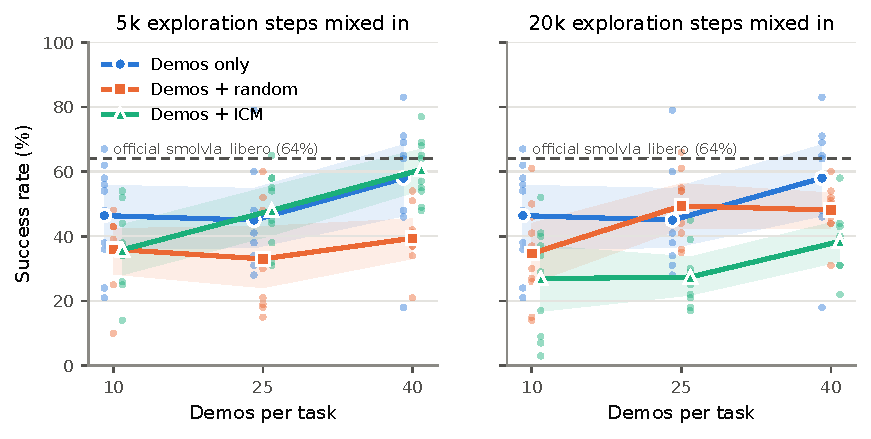
\includegraphics[width=\columnwidth]{fig_success_vs_demos.pdf}
\caption{Success versus demonstrations per task (mean of 10 seeds, 95\% CI).}
\label{fig:main}
\end{figure}
Fig.~\ref{fig:main}: demos only reaches 46, 45 and 58\% at 10, 25 and 40 demos (the public \texttt{smolvla\_libero} checkpoint scores 64\% on the same tasks). Pooled over demo budgets, mixing in exploration changes success by $-13.7$ [$-19.2$, $-7.8$] (random, 5k), $-5.7$ [$-11.1$, $-0.1$] (random, 20k), $-1.7$ [$-8.2$, $+5.4$] (ICM, 5k) and $-18.9$ [$-24.4$, $-13.2$] points (ICM, 20k), paired bootstrap 95\% intervals.

\subsection{Source effect and data-collection variance}
ICM minus random is $+12.0$ [$+7.5$, $+16.8$] points at 5k and $-13.2$ [$-17.3$, $-9.0$] at 20k. Fig.~\ref{fig:rep} shows independent re-collections: with 10 demos and 5k random steps, three collections give 36, 35 and 11\%. Every collection is below demos only. \pending{collection-level test with 3 collections per method, incl.\ ICM warm-up}

\begin{figure}[t]\centering
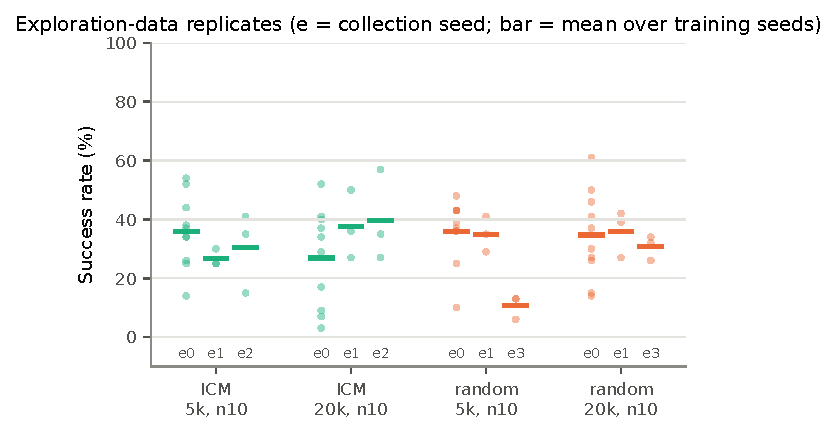
\includegraphics[width=\columnwidth]{fig_exploration_replicates.pdf}
\caption{Each point is a fine-tune; bars are means per exploration collection ($e$ = collection seed).}
\label{fig:rep}
\end{figure}

\subsection{Ablations and falsification tests}
\textbf{Mixing share.} At 10\% exploration frames success returns to the demos-only level; at 25--50\% it is lower (Fig.~\ref{fig:ratio}).
\textbf{Dilution control.} \pending{demos only at 10k steps vs 50\% mixes}.
\textbf{Exploration first.} \pending{10k steps on exploration, then 10k on demos, vs demos only 10k}.
\textbf{Trained curiosity.} \pending{ICM warm-up vs ICM vs random}.
\textbf{Action-chunk execution.} \pending{n\_action\_steps 10/25/50}.

\begin{figure}[t]\centering
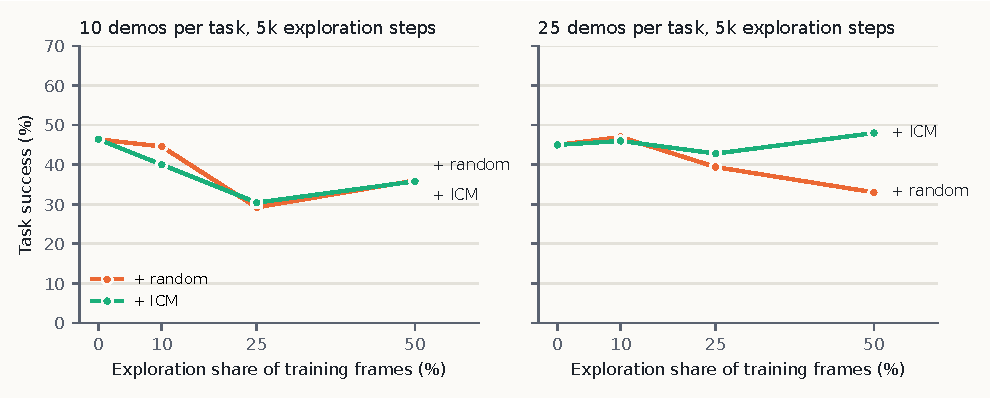
\includegraphics[width=\columnwidth]{fig_mixing_ratio.pdf}
\caption{Success versus exploration share of training frames (5k exploration steps).}
\label{fig:ratio}
\end{figure}

\subsection{Latency and memory}
\begin{table}[t]\centering\caption{Training and inference cost}\label{tab:cost}
\begin{tabular}{@{}lrr@{}}\toprule
GPU & s / step (bs 32) & 20k steps \\ \midrule
H100 PCIe & 0.172 & 0.96 h \\
H100 NVL & 0.183 & 1.02 h \\
A100 40GB & 0.283 & 1.57 h \\ \midrule
\multicolumn{3}{@{}l}{Peak training memory 7.75 GB; 100M / 450M params trainable} \\
\multicolumn{3}{@{}l}{Inference per 50-step chunk: \pending{ms} (\pending{GPU}), \pending{GB}} \\
\multicolumn{3}{@{}l}{Exploration: 20k steps in 32 min (rendering bound)} \\ \bottomrule
\end{tabular}
\end{table}
Table~\ref{tab:cost} summarizes cost from \pending{N} training logs and the inference profiler.

\section{Failure Analysis, Negative Results and Limitations}
\textbf{Why exploration data does not help here.} (1) SmolVLA fine-tunes only its action expert and state projection; the VLM is frozen, so exploration data cannot improve visual features. (2) Exploration actions are not predictable from observations (held-out $R^2\le0.01$, versus 0.42 for demonstrations), so a BC loss can only fit their marginal distribution. (3) Only 11--18\% of exploration frames come within 3\,cm of any demonstrated end-effector position. (4) A 50\% mix halves the demonstration gradient steps \pending{dilution-control result}.

\textbf{The first ICM explorer was barely trained.} With one PPO update per 2{,}560 steps it made 7 updates in 20k steps and its action standard deviation stayed at 1.00, so ``ICM'' differed from random mostly in action scale (mean $|a|$ 0.63 versus 0.50) and coverage (12.8k versus 10.2k 2-cm voxels). This is why the warm-up variant was added.

\textbf{Pseudo-replication.} In the main grid all seeds of a cell share one exploration collection, so seed-level intervals overstate certainty about the data source. Re-collections differ by up to 25 points.

\textbf{Rollout failures.} \pending{categorized failure modes from eval videos: missed grasp, wrong object, drop, timeout}.

\textbf{Limitations.} One suite and two tasks; one VLA with a frozen backbone; ICM as the only curiosity method; no inverse-dynamics or RL use of the data; simulation only.

\section{Conclusion and Future Work}
Adding task-free exploration data to SmolVLA fine-tuning with a behavior-cloning loss does not help and can cost up to 19 points; differences between exploration sources are within the variation between collections. The channel through which data enters training matters more than the explorer. Next steps: inverse-dynamics pretraining on the same data (as in TAP), unfreezing the VLM, stronger explorers (RND, trained ICM) and VLM-guided curiosity once a channel that carries value is found.

\begin{thebibliography}{10}
\bibitem{smolvla} M. Shukor et al., ``SmolVLA: A vision-language-action model for affordable and efficient robotics,'' arXiv:2506.01844, 2025.
\bibitem{libero} B. Liu et al., ``LIBERO: Benchmarking knowledge transfer for lifelong robot learning,'' NeurIPS Datasets and Benchmarks, 2023.
\bibitem{worldenv} J. Xiao et al., ``World-Env: Leveraging world model as a virtual environment for VLA post-training,'' arXiv:2509.24948, 2025.
\bibitem{tap} J. Shi et al., ``Learning to move before learning to do: Task-agnostic pretraining for VLAs,'' ICML, 2026, arXiv:2607.02466.
\bibitem{exorl} D. Yarats et al., ``Don't change the algorithm, change the data: Exploratory data for offline reinforcement learning,'' arXiv:2201.13425, 2022.
\bibitem{icm} D. Pathak et al., ``Curiosity-driven exploration by self-supervised prediction,'' ICML, 2017.
\bibitem{sensei} C. Sancaktar et al., ``SENSEI: Semantic exploration guided by foundation models to learn versatile world models,'' ICML, 2025.
\bibitem{dlr} R. Yang et al., ``Discover, learn, and reinforce: Scaling vision-language-action pretraining with diverse RL-generated trajectories,'' arXiv:2511.19528, 2025.
\bibitem{negtransfer} G. Xia et al., ``VLAFlow: A unified training framework for vision-language-action models via co-training and future latent alignment,'' arXiv:2607.01586, 2026.
\bibitem{fact} Q. Peng et al., ``FACT: Failure-aware causal training for world-action models,'' arXiv:2608.10232, 2026.
\end{thebibliography}
\end{document}
